% Notwendige Einstellung
  % Tools->Global Options-> Sweave: Weave Rnw files using: knitr
  %                                 Typeset LaTeX into PDF using: XeLaTeX (pdfLaTeX)
  
% Manuals: 
  % beamer-Dokumente: http://web.mit.edu/rsi/www/pdfs/beamer-tutorial.pdf
  % Sweave: https://rstudio-pubs-static.s3.amazonaws.com/188117_29a7a382c1884bd98ff54b9c7805613f.html
  % knitr: 
    %-Options: https://yihui.org/knitr/options/
 
  
%Tell R RStudio the path to latex // put behind "%" before "Compile PDF"
  %If you want RStudio to remember this command each time you start RStudio, you have to add the command to your .Rprofile file.
%Sys.setenv(PATH = paste(Sys.getenv("PATH"), "C:\\Program Files\\MiKTeX 2.9\\miktex\\bin\\x64", sep=.Platform$path.sep))
%Sys.setenv(PATH = paste(Sys.getenv("PATH"), "C:\\Users\\simon\\AppData\\Local\\Programs\\MIKTEX 2.9\\miktex\\bin\\x64", sep=.Platform$path.sep))

%install.packages('tinytex')
  %tinytex::install_tinytex()
  %tinytex:::install_yihui_pkgs()
  %tinytex::parse_packages(text = "! LaTeX Error: File `MnSymbol.sty' not found.")
  %tinytex::tlmgr_install("mnsymbol")

\documentclass[xcolor=dvipsnames]{beamer}\usepackage[]{graphicx}\usepackage[]{color}
% maxwidth is the original width if it is less than linewidth
% otherwise use linewidth (to make sure the graphics do not exceed the margin)
\makeatletter
\def\maxwidth{ %
  \ifdim\Gin@nat@width>\linewidth
    \linewidth
  \else
    \Gin@nat@width
  \fi
}
\makeatother

\definecolor{fgcolor}{rgb}{0.345, 0.345, 0.345}
\newcommand{\hlnum}[1]{\textcolor[rgb]{0.686,0.059,0.569}{#1}}%
\newcommand{\hlstr}[1]{\textcolor[rgb]{0.192,0.494,0.8}{#1}}%
\newcommand{\hlcom}[1]{\textcolor[rgb]{0.678,0.584,0.686}{\textit{#1}}}%
\newcommand{\hlopt}[1]{\textcolor[rgb]{0,0,0}{#1}}%
\newcommand{\hlstd}[1]{\textcolor[rgb]{0.345,0.345,0.345}{#1}}%
\newcommand{\hlkwa}[1]{\textcolor[rgb]{0.161,0.373,0.58}{\textbf{#1}}}%
\newcommand{\hlkwb}[1]{\textcolor[rgb]{0.69,0.353,0.396}{#1}}%
\newcommand{\hlkwc}[1]{\textcolor[rgb]{0.333,0.667,0.333}{#1}}%
\newcommand{\hlkwd}[1]{\textcolor[rgb]{0.737,0.353,0.396}{\textbf{#1}}}%
\let\hlipl\hlkwb

\usepackage{framed}
\makeatletter
\newenvironment{kframe}{%
 \def\at@end@of@kframe{}%
 \ifinner\ifhmode%
  \def\at@end@of@kframe{\end{minipage}}%
  \begin{minipage}{\columnwidth}%
 \fi\fi%
 \def\FrameCommand##1{\hskip\@totalleftmargin \hskip-\fboxsep
 \colorbox{shadecolor}{##1}\hskip-\fboxsep
     % There is no \\@totalrightmargin, so:
     \hskip-\linewidth \hskip-\@totalleftmargin \hskip\columnwidth}%
 \MakeFramed {\advance\hsize-\width
   \@totalleftmargin\z@ \linewidth\hsize
   \@setminipage}}%
 {\par\unskip\endMakeFramed%
 \at@end@of@kframe}
\makeatother

\definecolor{shadecolor}{rgb}{.97, .97, .97}
\definecolor{messagecolor}{rgb}{0, 0, 0}
\definecolor{warningcolor}{rgb}{1, 0, 1}
\definecolor{errorcolor}{rgb}{1, 0, 0}
\newenvironment{knitrout}{}{} % an empty environment to be redefined in TeX

\usepackage{alltt}
\mode<presentation>{\usetheme{Goettingen}}

\usepackage[utf8]{inputenc}
\usepackage{babel} %eigentlich: [ngerman]{babel}
%\usepackage{amsmath} not needed because loaded by mathtools
\usepackage{mathtools} % use of \underbrace{} & \overbrace{} (-> https://ctan.net/obsolete/info/math/voss/mathmode/Mathmode.pdf | Loads amsmath
\usepackage{MnSymbol} % Für Unabhängigkeitssymbol
\usepackage{eurosym} % for \euro -> Euro Symbol
\usepackage{url} % for \url{} to include urls in text
\usepackage{graphicx,grffile} % graphicx: for includegraphics{} // grffile: supports multiple dots and spaces in filenames



%\usepackage{tcolorbox} % includes \tcboxverb{}-command to mark code in text
%\tcbuselibrary{xparse}

%\usepackage[width=5.05cm]{geometry}
%\usepackage{color,soul}

%\codebox{}-command
%\colorlet{codecolor}{black!30}
%\newcommand{\codebox}[1]{%
%  \colorbox{codecolor}{\ttfamily \detokenize{#1}}%
%}



%Seitenzahl unten links anzeigen
  \defbeamertemplate*{footline}{split theme} 
  {% 
    \leavevmode% 
    \hbox{
    \begin{beamercolorbox}[wd=.5\paperwidth,ht=2.5ex,dp=1.125ex,leftskip=.3cm,rightskip=.3cm plus1fil]{title in head/foot}%                                            %selbst eingefügte Zeile 
      \insertframenumber{} / \inserttotalframenumber  %selbst eingefügte Zeile 
    \end{beamercolorbox}}% 
    \vskip0pt% 
  } 

%Numbering sections in table of content
  \setbeamertemplate{section in toc}[sections numbered]
  \setbeamertemplate{subsection in toc}[subsections numbered]

%About the document
  \author{Simon Ress}
  \institute{Ruhr-Universität Bochum}
  \title{Workshop Web-Scraping in R}
  %\subtitle{Modern Causal Analysis. Rubin Causal Model und Directed Acyclic Graphs} 
  \date{15.02.2020}

%Seite mit Chapter Name vor jedem Chapter erstellen
  \AtBeginSection[]{
      \begin{frame}
      \vfill
      \centering
      \begin{beamercolorbox}[sep=8pt,center,shadow=true,rounded=true]{section page}
          \usebeamerfont{title}%
          \textit{Chap. \thesection~}%
                  {\color{black} \insertsectionhead}\par%
      \end{beamercolorbox}
      \vfill
      \end{frame}
  }


%\usepackage{listings} % for line break in chunks





\IfFileExists{upquote.sty}{\usepackage{upquote}}{}
\begin{document}
%\SweaveOpts{concordance=TRUE}

\maketitle

%Inhaltsverzeichnis
\begin{frame}
\frametitle{Inhalt} 
\tableofcontents
\end{frame}


%-------------------------------------------------------------%
%------------------------- Übersicht -------------------------%
%-------------------------------------------------------------%

\section{Übersicht} % Wichtig für Inhaltsverzeichnis

\begin{frame}{Übersicht Web-Scraping}
  \begin{figure}
  	\centering
  	\caption{Schema von Web-Scraping \& zentrale Befehle}
  	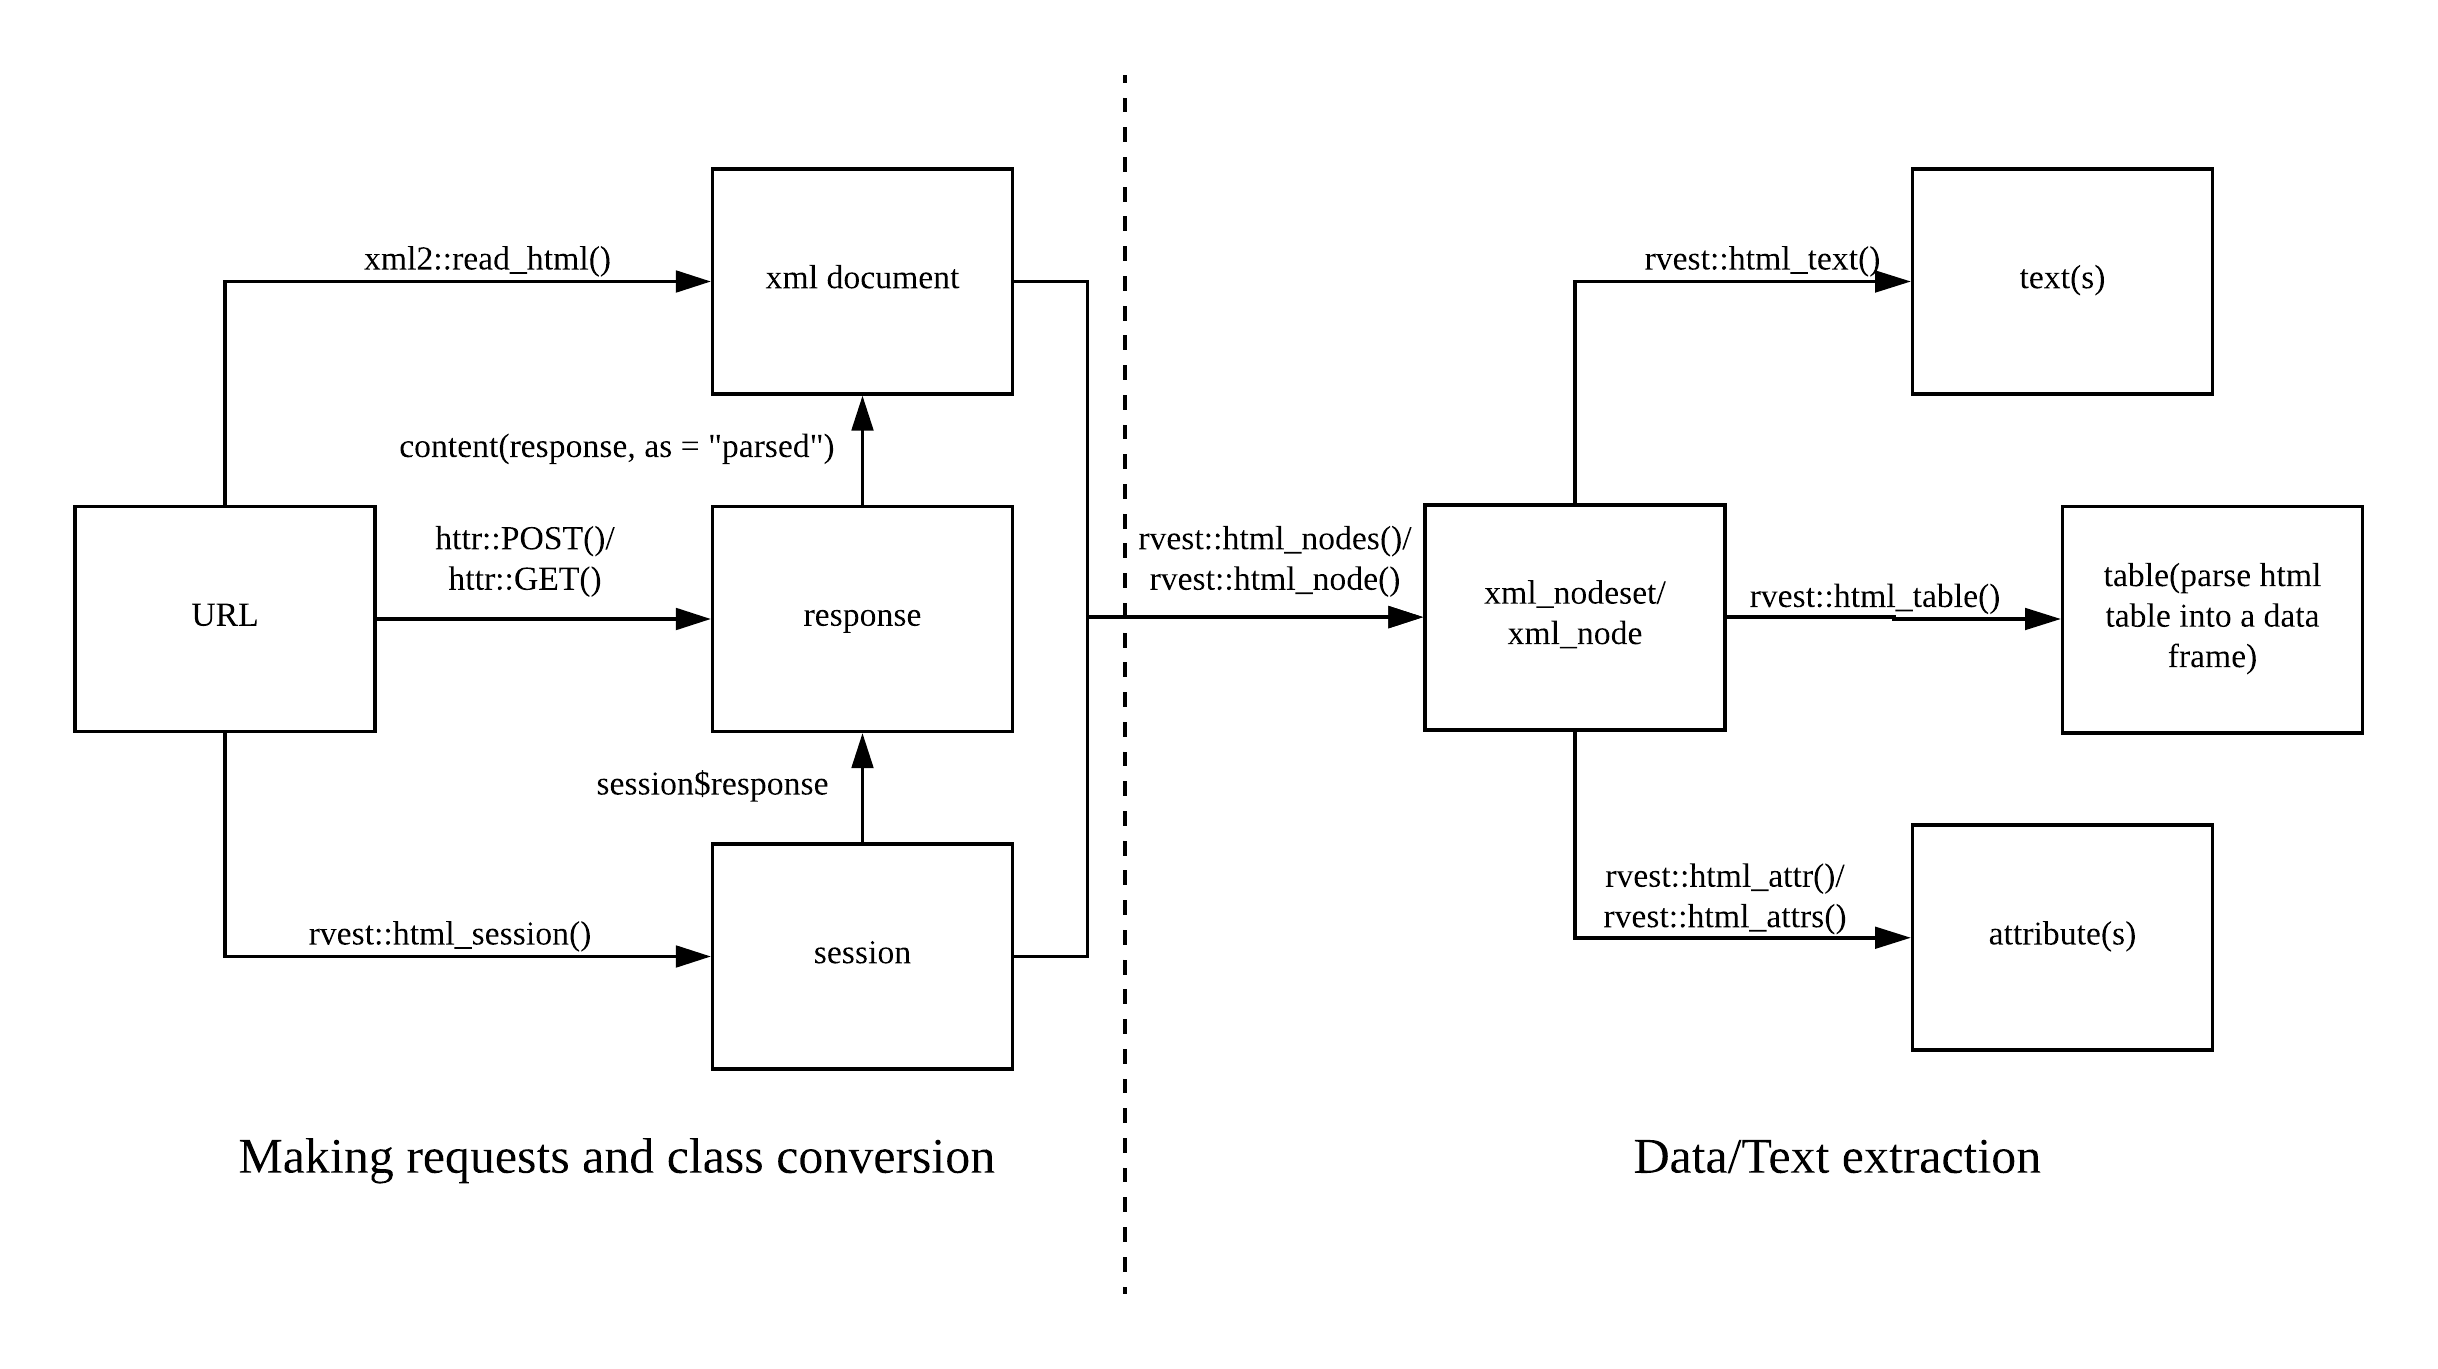
\includegraphics[width=1\textwidth]{figure/overview-web-scraping.png}
  	{\footnotesize \tiny Quelle: https://github.com/yusuzech/r-web-scraping-cheat-sheet \par}
  \end{figure}
\end{frame}



\section{HTML} % Wichtig für Inhaltsverzeichnis


\begin{frame}{HTML: Was ist das?}
\begin{itemize}
  \item Hypertext Markup Language (HTML) ist eine textbasierte Auszeichnungssprache 
  \item Dient der Strukturierung von Webseiten
  \item Besteht aus einer Reihe von Elementen ($\rightarrow$ definieren Struktur)
  \item Elemente regeln die Darstellung durch den Browser
  \item Elemente bestimmen; "das ist eine Überschrift", "das ist ein Paragraph", "das ist ein Link" usw.
\end{itemize}
\end{frame}


%------------------------------------------------------------------------------------------------%
%------------------------------------------------------------------------------------------------%


\begin{frame}[fragile]{HTML: Elemente, Tags und Attribute I}
\small

\begin{itemize}
\item \textbf{Tags:} Start- ({\color{gray}{\textbf{$<$Tag-Name$>$}}}) und End-Punkte ({\color{gray}{\textbf{$<$/Tag-Name$>$}}}) von Elementen. 
\item \textbf{Element:} Zusammenspiel aus darzustellendem Inhalt und Darstellungsvorgabe für Browser
\end{itemize}
\[ 
\overbrace{
  \begingroup
    \color{red}
    \underbrace{<h1>}_\text{(Start-)Tag} 
  \endgroup
  \begingroup
    \color{blue}
    \underbrace{$HTML Inhalte$}_\text{Inhalt} 
  \endgroup
  \begingroup
    \color{red}
    \underbrace{</h1>}_\text{(End-)Tag}
  \endgroup
}^\text{Element}
\]

\end{frame}


%------------------------------------------------------------------------------------------------%
%------------------------------------------------------------------------------------------------%


\begin{frame}[fragile]{HTML: Elemente, Tags und Attribute II}
\small
\begin{itemize}
\item \textbf{Attribute:} Optionen der Elemente, welche in Start-Tags definiert werden (bestehen aus Attribut-Name \& -Wert)
\end{itemize}
\scriptsize
\[ 
\underbrace{
  \begingroup
    \color{red}
    \underbrace{
      <
      {\color{Maroon}\underbrace{a}_{\mathclap{Tag-Name}}}
      {\color{Green}\overbrace{
        {\color{YellowGreen}\overbrace{href}^{\mathclap{Attribut-Name}}}=
        {\color{SpringGreen}\overbrace{https://www.w3schools.com/tags/ref\_byfunc.asp}^\text{Attribut-Wert}}
      }^{\mathclap{Attribute}}}
    >}_\text{(Start-)Tag}
  \endgroup
  \begingroup
    \color{blue}
    hier
  \endgroup
  \begingroup
    \color{red}
    \underbrace{</a>}_\text{(End-)Tag}
  \endgroup
}_\text{Element}
\]

\end{frame}



\begin{frame}{HTML: Grundstruktur}
\textbf{Ein HTML-Dokument besteht aus drei Bereichen:}
\begin{itemize}
\item \textbf{Dokumenttypdeklaration ({\color{gray}{\textbf{$<$!DOCTYPE html$>$}}}):} Beginn der Datei, die die verwendete Dokumenttypdefinition (DTD) angibt, z. B. HTML oder CSS
\item \textbf{HTML-Kopf ({\color{gray}{\textbf{$<$head$>$}}}):} Enthält hauptsächlich technische oder dokumentarische Informationen, die üblicherweise nicht im Anzeigebereich des Browsers dargestellt werden
\item \textbf{HTML-Körper ({\color{gray}{\textbf{$<$body$>$}}}):} Enthält alle Informationen die gewöhnlich im Anzeigebereich des Browsers zu sehen sind
\end{itemize}
\end{frame}


\begin{frame}{HTML: Grafik der Grundstruktur }
  \begin{figure}
  	\centering
  	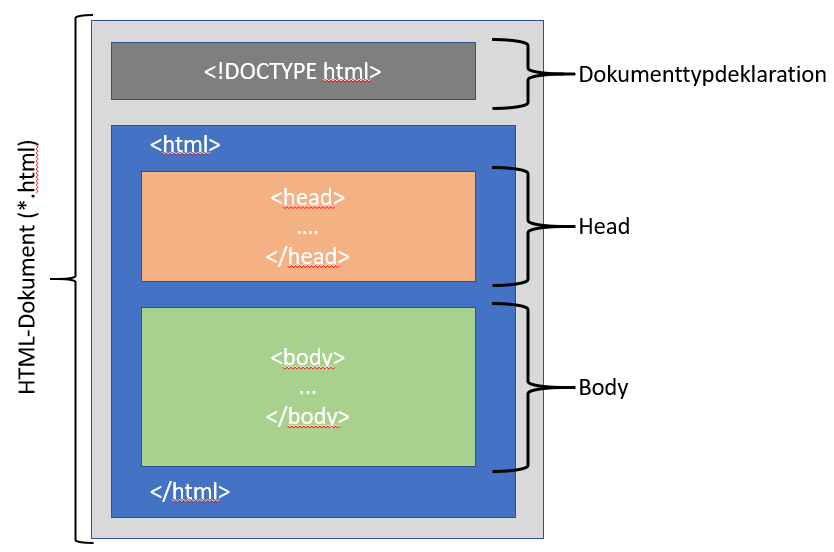
\includegraphics[width=0.9\textwidth]{figure/htmlbasicstructure.png}
  	\\
  	{\footnotesize \tiny Quelle: Eigene Darstellung \par}
  \end{figure}
\end{frame}





\begin{frame}{HTML: Überblick von Elementen}

\begin{table}[]
\begin{tabular}{ll}
\hline
\textbf{Element-Name}                                                              & \textbf{Beschreibung}               \\ \hline
{\color{gray}{\textbf{$<$title$>$}}}                                                     & Titel des Dokuments                 \\ \hline
{\color{gray}{\textbf{$<$h1$>$}}} bis {\color{gray}{\textbf{$<$h6$>$}}}                          & Überschriften in absteigender Ebene \\ \hline
{\color{gray}{\textbf{$<$p$>$}}}                                                         & Paragraph                       \\ \hline
{\color{gray}{\textbf{$<$b$>$}}}, {\color{gray}{\textbf{$<$i$>$}}}, {\color{gray}{\textbf{$<$u$>$}}} & Text fett, kursiv, unterstrichten   \\ \hline
{\color{gray}{\textbf{$<$a$>$}}}                                                         & Hyperlink                           \\ \hline
{\color{gray}{\textbf{$<$ul$>$}}} / {\color{gray}{\textbf{$<$ol$>$}}}                           & Ungeordnete / geordnete Liste        \\ \hline
{\color{gray}{\textbf{$<$li$>$}}}                                                       & Item einer Liste                 \\ \hline
{\color{gray}{\textbf{$<$picture$>$}}}                                                   & Bild einfügen                       \\ \hline
{\color{gray}{\textbf{$<$video$>$}}}                                                     & Video einfügen (Medien Element)     \\ \hline
{\color{gray}{\textbf{$<$audio$>$}}}                                                    & Sound einfügen (Medien Element)     \\ \hline
{\color{gray}{\textbf{$<$source$>$}}}                                                    & Datei für Medien Element           
\end{tabular}
\end{table}


\href{https://www.w3schools.com/tags/ref_byfunc.asp}{\textbf{Hier}} eine ausführliche Liste von HTML-Elementen nach Verwendungszweck. 
\end{frame}


\begin{frame}{HTML: Basics.html (Schema)}
  \begin{figure}
  	\centering
  	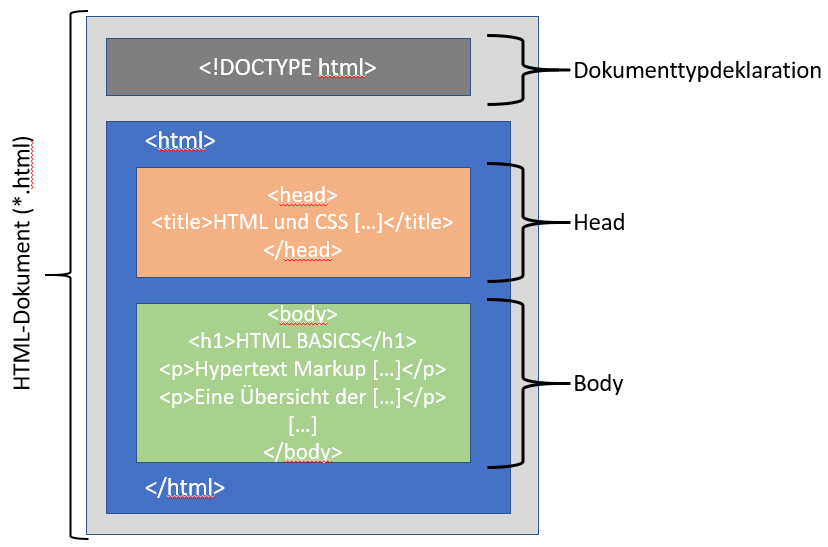
\includegraphics[width=0.9\textwidth]{figure/BasicHtml(Schema).png}
  	\\
  	\floatfoot{\tiny Quelle: Eigene Darstellung}
  \end{figure}
\end{frame}


\begin{frame}[fragile]{HTML: Basics.html (Code)}
\begin{knitrout}\tiny
\definecolor{shadecolor}{rgb}{0.969, 0.969, 0.969}\color{fgcolor}\begin{kframe}
\begin{alltt}
<!DOCTYPE html>
  <html>
    <head>
      <title>HTML und CSS Einführung</title>
    </head>
  
    <body>
      <h1>HTML BASICS</h1>
      <p>Hypertext Markup \hlkwd{Language} (HTML) ist eine
         textbasierte Auszeichnungssprache zur 
         Strukturierung elektronischer Dokumente</p>
      <p>Eine Übersicht der verschiedenen HTML-
         Elemente findet sich <a href="
         https://www.w3schools.com/tags/ref_byfunc.asp"
         >hier</a>.</p>
      [...]
    </body>
  </html>
\end{alltt}
\end{kframe}
\end{knitrout}
\end{frame}


\begin{frame}{HTML: Basics.html (Browser)}
  \begin{figure}
  	\centering
  	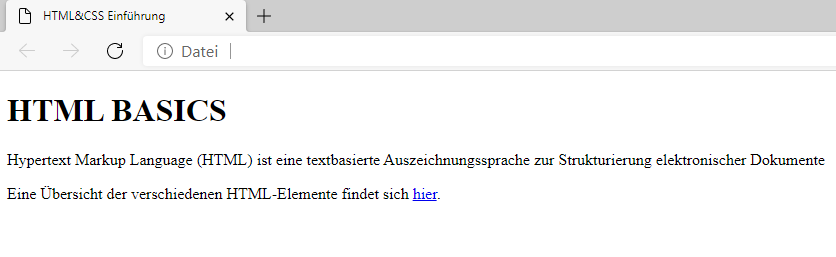
\includegraphics[width=1\textwidth]{figure/BasicHtml(Browser).png}
  	\floatfoot{\tiny Quelle: Darstellung in Chrome Version 88.0.4324.182 (Offizieller Build) (64-Bit)}
  \end{figure}
  Link: \href{www.resssis4.io.noc.ruhr-uni-bochum.de/homepage}{www.resssis4.io.noc.ruhr-uni-bochum.de/homepage} 
\end{frame}


\begin{frame}{HTML: Baumstruktur}
Die Verschachtelung der Inhalte eines HTML-Dokuments kann am besten mittels eines Baumdiagramms dargestellt werden. 
\begin{figure}
  	\centering
  	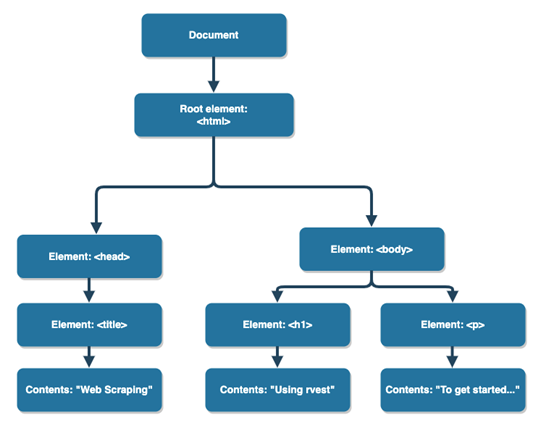
\includegraphics[width=0.7\textwidth]{figure/HTMLtree.png}
  \end{figure}
\end{frame}


\section{CSS}

\begin{frame}{CSS-Grundlagen}
\begin{itemize}
\item Cascading Style Sheets (CSS) ist eine Stylesheet-Sprache für elektronische Dokumente und zusammen mit HTML und JavaScript eine der Kernsprachen des World Wide Webs.
\item CSS wurde entworfen, um Darstellungsvorgaben weitgehend von den Inhalten zu trennen.
\item Layouts, Farben und Typografie von Websites können mit Cascade Style Sheets formatiert
werden (Trennung von Inhalte=HTML/XML und Layout=CSS)
\item Speicherung in separaten CSS-Dateien
\item Darstellung von immer wiederkehrenden HTML-Inhalten erleichtert werden, indem Stile, Farbe und Formen für Titel, Schriftgröße usw. definiert werden können
\item Aufbau nach id, class \& attribute
\end{itemize}
\end{frame}


\begin{frame}[fragile]{CSS-Struktur}
\textbf{Aufbau einer CSS-Anweisung:}
\begin{kframe}
\begin{alltt}
Selektor1 [, Selektor2 [, …] ] \{
    Eigenschaft-1: Wert-1;
    …
    Eigenschaft-n: Wert-n[;]
\}
/* Kommentar */
/* Optionale Angaben in eckigen Klammern */
\end{alltt}
\end{kframe}
\end{frame}


\begin{frame}[fragile]{CSS-Struktur: Beispiel}
\textbf{Beispiel einer CSS-Anweisung:}
\begin{kframe}
\begin{alltt}
p.info \{ \hlcom{#ID:p // class: info}
  font-family: arial, sans-serif;
  line-height: 150%;
  margin-left: 2em;
  padding: 1em;
  border: 3px solid red;
  background-color: \hlcom{#f89;}
  display: inline-block;
\}
p.info span \{
  font-weight: bold;
\}
p.info span::after \{
  content: \hlstr{": "};
\}
\end{alltt}
\end{kframe}
\end{frame}


\begin{frame}[fragile]{Einbindung von CSS in HTML}
\textbf{HTML-Code:}
\begin{kframe}
\begin{alltt}
<p class=\hlstr{"info"}>
  <span>Hinweis</span>
  Sie haben sich erfolgreich angemeldet.
</p>
\end{alltt}
\end{kframe}
\textbf{Ergebnis im Browser:}  
  \begin{figure}
  	\centering
  	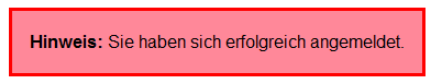
\includegraphics[width=0.7\textwidth]{figure/CSSinHTML.png}
  	\\
  	\floatfoot{\tiny Quelle: Eigene Darstellung}
  \end{figure}
\end{frame}


\begin{frame}[fragile]{CSS: id, class \& attribute}
\textbf{HTML-Code:}
\begin{kframe}
\begin{alltt}
<div class=\hlstr{"hallo-beispiel"}>
    <a href=\hlstr{"contact.html"}>Contact us:</a>
    <span lang=\hlstr{"en-us en-gb en-au en-nz"}>
      Hallo Welt!
    </span>
</div>
\end{alltt}
\end{kframe}
  \begin{figure}
  	\centering
  	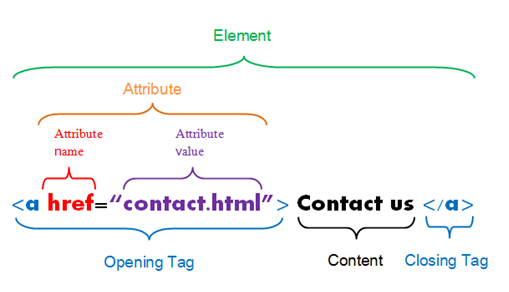
\includegraphics[width=0.6\textwidth]{figure/CSSStructure.png}
  	\\
  	\floatfoot{\tiny Quelle: Eigene Darstellung}
  \end{figure}
\end{frame}



\begin{frame}{CSS-Selector}
In CSS sind selectors Muster, mit denen die Elemente ausgewählt werden, die abgefragt werden sollen.\\
Hier ein erster Einblick: \href{https://www.w3schools.com/cssref/trysel.asp}{CSS Selector Tester}
\end{frame}


\begin{frame}{CSS-Selector: Übersicht I}
\begin{table}[]
\footnotesize
\begin{tabular}{lll}
\textbf{Selector}                             & \textbf{Beispiel} & \textbf{Beschreibung}                                                                                                                 \\ \hline
\textit{.class}                               & .intro            & Alle Elemente mit class="intro"                                                                                                       \\ \hline
\textit{.class1.class2}                       & .name1.name2      & \begin{tabular}[c]{@{}l@{}}Alle Elemente mit "name1" \& \\ "name2" in class attribute\end{tabular}                                    \\ \hline
\textit{.class1 .class2}                      & .name1 .name2     & \begin{tabular}[c]{@{}l@{}}Alle Elemente mit class="name2"\\ welche Elementen mit \\ class="name1" untergeordnet \\ sind\end{tabular} \\ \hline
\textit{\#id}                                 & \#firstname       & Alle Elemente mit id="firstname"                                                                                                      \\ \hline
\textit{*}                                    & *                 & Alle Elemente                                                                                                                         \\ \hline
\textit{element}                              & p                 & Alle \textless{}p\textgreater Elemente                                                                                                \\ \hline
\textit{element.class} & p.intro           & \begin{tabular}[c]{@{}l@{}}Alle \textless{}p\textgreater Elemente mit \\ class="intro"\end{tabular}                                  
\end{tabular}
\end{table}
\end{frame}



\begin{frame}{CSS-Selector: Übersicht II}
\begin{table}[]
\footnotesize
\begin{tabular}{lll}
\textbf{Selector}                       & \textbf{Beispiel}                     & \textbf{Beschreibung}                                                                                                                   \\ \hline
element\textgreater{}element            & div \textgreater p                    & \begin{tabular}[c]{@{}l@{}}Alle Elemente \textless{}p\textgreater deren \\ parent \textless{}div\textgreater Elemente sind\end{tabular} \\ \hline
element\textgreater{}element            & div  p                                & \begin{tabular}[c]{@{}l@{}}Alle \textless{}p\textgreater{}-Elemente in \\ \textless{}div\textgreater{}-Elementen\end{tabular}           \\ \hline
{[}attribute{]}                         & {[}target{]}                          & \begin{tabular}[c]{@{}l@{}}Alle Elemente mit \\ target attribute\end{tabular}                                                           \\ \hline
{[}attribute=value{]}                   & {[}target=\_blank{]}                  & \begin{tabular}[c]{@{}l@{}}Alle Elemente mit \\ target=\_blank\end{tabular}                                                             \\ \hline
{[}attribute\textasciicircum{}=value{]} & a{[}href\textasciicircum{}="https"{]} & \begin{tabular}[c]{@{}l@{}}Alle Elemente deren href \\ attribute mit "https" beginnt\end{tabular}                                       \\ \hline
{[}attribute\$=value{]}                 & a{[}href\$=".pdf"{]}                  & \begin{tabular}[c]{@{}l@{}}Alle Elemente deren href \\ attribute mit ".pdf" endet\end{tabular}                                          \\ \hline
{[}attribute*=value{]}                  & a{[}href*="w3"{]}                     & \begin{tabular}[c]{@{}l@{}}Alle Elemente deren href \\ attribute "w3" enthält\end{tabular}                                             
\end{tabular}
\end{table}
\end{frame}



\begin{frame}{CSS-Selector \& XPaths}
\footnotesize
\begin{table}[]
\footnotesize
\begin{tabular}{lll}
\hline
\textbf{Ziel}                              & \textbf{CSS-Selektor}                 & \textbf{XPath}                           \\ \hline
All Elements                      & *                            & //*                             \\ \hline
All Elements: p                   & p                            & //p                             \\ \hline
All Child Elements of p           & p \textgreater *             & //p/*                           \\ \hline
All Elements with ID foo          & \#foo                        & //*{[}@id='foo'{]}              \\ \hline
All Elements with class foo       & .foo                         & //*{[}contains(@class, 'foo')   \\ \hline
All Elements with attribute title & *{[}title{]}                 & //*{[}@title{]}                 \\ \hline
First Child of all p              & p\textgreater{}*:first-child & //p/*{[}0{]}                    \\ \hline
All Elements p with Child a       & \textit{Not possible}        & //p{[}a{]}                      \\ \hline
Next Element                      & p + *                        & //p/follow-sibling::*{[}0{]}    \\ \cline{1-1} \cline{3-3} 
Previous Element                  & \textit{Not possible}        & //p/preceding-sibling::*{[}0{]} \\ \hline
\end{tabular}
\end{table}
\end{frame}



\section{XPaths}

\begin{frame}{XPath}
\begin{itemize}
\item XML Path Language (XPath) ist eine Abfragesprache, um Teile eines XML-Dokumentes zu adressieren und auszuwerten
\item Seit HTML5 ist die Struktur von HTML-Dokumenten äquivalent zu XML-Dokumenten
\item XPath-Ausdruck adressiert Teile eines XML-Dokuments, das dabei als Baum betrachtet wird
\end{itemize}
\textbf{Schema eines XML-Dokuments}
  \begin{figure}
	\centering
	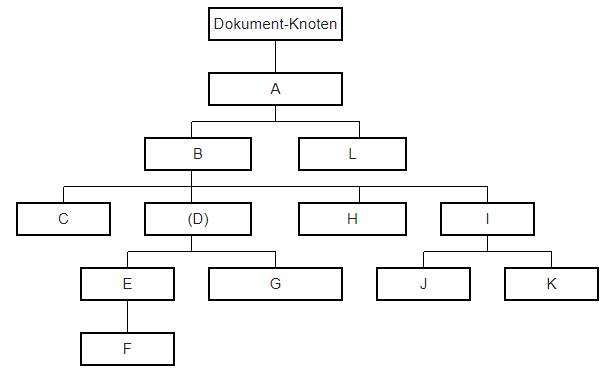
\includegraphics[width=0.6\textwidth]{figure/XML-Structure.png}
	\floatfoot{\tiny Quelle: Eigene Darstellung}
  \end{figure}
\end{frame}


\begin{frame}{XPath-Nodes}
\textbf{XPath-Nodes}\\
In XPath gibt es sieben Arten von Knoten: element, attribute, text, namespace, processing-instruction, comment, and document nodes

XML-Dokumente werden als Bäume von nodes behandelt. Das oberste Element des Baums wird als root-Element (Stammelement) bezeichnet.
\end{frame}


\begin{frame}[fragile]{XPath-Nodes}
\textbf{Beispiel}
\begin{kframe}
\begin{alltt}
<?xml version=\hlstr{"1.0"} encoding=\hlstr{"UTF-8"}?>

<bookstore>
  <book>
    <title lang=\hlstr{"en"}>Harry Potter</title>
    <author>J K. Rowling</author>
    <year>2005</year>
    <price>29.99</price>
  </book>
</bookstore>
\end{alltt}
\end{kframe}
  \begin{itemize}
    \item Root-Element node: <bookstore>
    \item Element node: $<$author$>$ J K. Rowling $<$/author$>$
    \item Attribute node: lang="en" 
  \end{itemize}
\end{frame}


\begin{frame}[fragile]{Beziehungen zwischen Nodes: parent}
Jedes Element und Attribut hat ein übergeordnetes Element (parent).\\
Im folgenden Beispiel ist das $<$book$>$ element das übergeordnete Element von $<$title$>$, $<$author$>$, $<$year$>$ und $<$price$>$:
\begin{kframe}
\begin{alltt}
<book>
  <title>Harry Potter</title>
  <author>J K. Rowling</author>
  <year>2005</year>
  <price>29.99</price>
</book>
\end{alltt}
\end{kframe}
\end{frame}


\begin{frame}[fragile]{Beziehungen zwischen Nodes: children}
Nodes-Elemente können null, ein oder mehrere children (untergeordnete Knoten) haben. \\
Im folgenden Beispiel sind $<$title$>$, $<$author$>$, $<$year$>$ und $<$price$>$ alle untergeordnete Elemente des $<$book$>$-Elements:
\begin{kframe}
\begin{alltt}
<book>
  <title>Harry Potter</title>
  <author>J K. Rowling</author>
  <year>2005</year>
  <price>29.99</price>
</book>
\end{alltt}
\end{kframe}
\end{frame}


\begin{frame}[fragile]{Beziehungen zwischen Nodes: siblings}
Nur Nodes mit dem selben parent (übergeordneten Element). \\
Im folgenden Beispiel: $<$title$>$, $<$author$>$, $<$year$>$ und $<$price$>$
\begin{kframe}
\begin{alltt}
<book>
  <title>Harry Potter</title>
  <author>J K. Rowling</author>
  <year>2005</year>
  <price>29.99</price>
</book>
\end{alltt}
\end{kframe}
\end{frame}


\begin{frame}[fragile]{Beziehungen zwischen Nodes: ancestors}
Alle parent-Elemente einer Node und deren parent. \\
Im folgenden Beispiel sind $<$book$>$ und $<$bookstore$>$ die ancestors von $<$title$>$
\begin{kframe}
\begin{alltt}
<bookstore>
  <book>
    <title>Harry Potter</title>
    <author>J K. Rowling</author>
    <year>2005</year>
    <price>29.99</price>
  </book>
</bookstore>
\end{alltt}
\end{kframe}
\end{frame}


\begin{frame}[fragile]{Beziehungen zwischen Nodes: descendants}
Alle child-Elemente einer Node und deren child \\
Im folgenden Beispiel sind $<$book$>$, $<$title$>$, $<$author$>$, $<$year$>$ und $<$price$>$ die descendants von $<$bookstore$>$
\begin{kframe}
\begin{alltt}
<bookstore>
  <book>
    <title>Harry Potter</title>
    <author>J K. Rowling</author>
    <year>2005</year>
    <price>29.99</price>
  </book>
</bookstore>
\end{alltt}
\end{kframe}
\end{frame}


\begin{frame}{Syntax zur Auswahl von Nodes}
XPath verwendet Pfadausdrücke, um Nodes in einem XML-Dokument auszuwählen. Die Node wird ausgewählt, indem einem Pfad oder Schritten gefolgt wird. Hier die nützlichsten Pfadausdrücke:

\begin{table}[]
\begin{tabular}{ll}
\textbf{Ausdruck} & \textbf{Beschreibung}                                                                                                     \\ \hline
\textit{nodename}   & \begin{tabular}[c]{@{}l@{}}Auswahl aller Nodes mit dem \\ Namen "nodename"\end{tabular}                                  \\ \hline
/                   & Auswahl der root-Node                                                                                                    \\ \hline
//                  & \begin{tabular}[c]{@{}l@{}}Auswahl von Nodes innerhalb \\ der aktuellen Node, welche der \\ Auswahl entspricht\end{tabular} \\ \hline
.                   & Auswahl der aktuellen Node                                                                                               \\ \hline
..                  & Auswahl des parent der aktuellen Node                                                                                    \\ \hline
@                   & Auswahl von attributes                                                                                                  
\end{tabular}
\end{table}

\end{frame}



\begin{frame}{Prädikate zur Auswahl von Nodes}
Prädikate werden verwendet, um eine bestimmte Node oder eine Node mit einen bestimmten Wert zu finden. \\
Prädikate werden immer in eckige Klammern gesetzt.

\begin{table}[]
\footnotesize
\begin{tabular}{lll}
\textbf{Pfadausdruck}                  & \textbf{Beschreibung}                                                                                                                        &  \\ \cline{1-2}
nodename{[}1{]}                        & \begin{tabular}[c]{@{}l@{}}Wählt das erste Element mit \\ entsprechendem Namen aus\end{tabular}                                              &  \\ \cline{1-2}
nodename{[}last(){]}                   & \begin{tabular}[c]{@{}l@{}}Wählt das letzte Element mit \\ entsprechendem Namen aus\end{tabular}                                             &  \\ \cline{1-2}
nodename{[}last()-1{]}                 & Wählt das vorletzte Element aus                                                                                                              &  \\ \cline{1-2}
nodename{[}position()\textless{}3{]}   & \begin{tabular}[c]{@{}l@{}}Wählt die ersten beiden \\ Element aus\end{tabular}                                                               &  \\ \cline{1-2}
nodename{[}@lang{]}                    & \begin{tabular}[c]{@{}l@{}}Wählt alle entsprechenden Elemente\\ mit einem attribut lang aus\end{tabular}                                     &  \\ \cline{2-2}
nodename{[}@lang='en'{]}               & \begin{tabular}[c]{@{}l@{}}Wählt alle entsprechenden Elemente\\ aus, bei denen das attribute lang den \\ Wert 'en' hat\end{tabular}          &  \\ \cline{1-2}
nodename{[}price\textgreater{}35.00{]} & \begin{tabular}[c]{@{}l@{}}Wählt alle entsprechenden Elemente\\ aus, die ein price Element mit einem\\ Wert von größer 35 haben\end{tabular} & 
\end{tabular}
\end{table}
\end{frame}



\begin{frame}[fragile]{Übung zu XPaths}
\begin{kframe}
\begin{alltt}
<?xml version=\hlstr{"1.0"} encoding=\hlstr{"utf-8"} standalone=\hlstr{"yes"} ?>
<dok>
    <!-- ein XML-Dokument -->
    <kap title=\hlstr{"Nettes Kapitel"}>
        <pa>Ein Absatz</pa>
        <pa>Noch ein Absatz</pa>
        <pa>Und noch ein Absatz</pa>
        <pa>Nett, oder?</pa>
    </kap>
    <kap title=\hlstr{"Zweites Kapitel"}>
        <pa>Ein Absatz</pa>
        <pa format=\hlstr{"bold"}>Erste Zeile</pa>
        <pa format=\hlstr{"bold"}>Zweite Zeile</pa>
        <pa format=\hlstr{"italic"}>Dritte Zeile</pa>
    </kap>
</dok>
\end{alltt}
\end{kframe}
\end{frame}


%-------------------------------------------------------------%
%--------------------------- Rvest ---------------------------%
%-------------------------------------------------------------%

\section{Rvest} % Wichtig für Inhaltsverzeichnis


\begin{frame}{Was ist Rvest?}
Das Packet \textit{rvest} macht es einfach Daten von Webseiten (HTML \& XML) zu extrahiert (web scraping) und zu manipulieren. Es wurde für die Arbeit mit dem Packet \textit{magrittr} (Pipe-Operator: \%$>$\%) entwickelt, um die Syntax für gängiger Web-Scraping-Aufgaben zu vereinfachen
\end{frame}


\begin{frame}{Grundlegende Funktionen}
Nachdem einlesen eines HTML-Dokuments mit read\_html():
  \begin{itemize}
  \item Auswahl eines Teils des Dokuments mittel 'CSS-Selectors': html\_nodes() 
  \item Extraktion von bestimmten Komponenten:
    \begin{itemize}
      \item html\_name() (Namen des tag)
      \item html\_text() (Gesamter Text im tag)
      \item html\_attr() (Ausprägung eines 'attribute')
      \item html\_attrs() (Alle 'attributes')
    \end{itemize}
  \item Tabellen in einen Datensatz ''parsen'': html\_table()
  \item Navigieren auf der Webseite: back(), forward()
  \end{itemize}
\end{frame}


\begin{frame}[fragile]{Erste Schritte mit Rvest}
\textbf{Webseite einlesen und filtern}
\begin{knitrout}\tiny
\definecolor{shadecolor}{rgb}{0.969, 0.969, 0.969}\color{fgcolor}\begin{kframe}
\begin{alltt}
\hlcom{#Install and load the package/library}
  \hlkwa{if}\hlstd{(}\hlopt{!}\hlkwd{require}\hlstd{(}\hlstr{"rvest"}\hlstd{))} \hlkwd{install.packages}\hlstd{(}\hlstr{"rvest"}\hlstd{)}
  \hlkwd{library}\hlstd{(rvest)}

\hlcom{#Start by reading a HTML page}
  \hlstd{starwars} \hlkwb{<-} \hlkwd{read_html}\hlstd{(}\hlstr{"https://rvest.tidyverse.org/articles/starwars.html"}\hlstd{)}

\hlcom{#Get an overview of the structure}
  \hlstd{films} \hlkwb{<-} \hlstd{starwars} \hlopt \hlkwd{html_nodes}\hlstd{(}\hlstr{"section"}\hlstd{)}
  \hlstd{films}

\hlcom{#Extract the movies' names /extract one element per film}
  \hlstd{title} \hlkwb{<-} \hlstd{films} \hlopt
    \hlkwd{html_node}\hlstd{(}\hlstr{"h2"}\hlstd{)} \hlopt
    \hlkwd{html_text}\hlstd{(.,} \hlkwc{trim} \hlstd{=} \hlnum{TRUE}\hlstd{)}
  \hlstd{title}

\hlstd{episode} \hlkwb{<-} \hlstd{films} \hlopt
  \hlkwd{html_node}\hlstd{(}\hlstr{"h2"}\hlstd{)} \hlopt
  \hlkwd{html_attr}\hlstd{(}\hlstr{"data-id"}\hlstd{)} \hlopt
  \hlkwd{as.numeric}\hlstd{()}
\hlstd{episode}
\end{alltt}
\end{kframe}
\end{knitrout}
\end{frame}



\begin{frame}[fragile]{Tabellen einlesen}
Wenn die Seite tabellarische Daten enthält, können diese mit html\_table() direkt in einen Datensatz konvertiert werden.
\begin{knitrout}\tiny
\definecolor{shadecolor}{rgb}{0.969, 0.969, 0.969}\color{fgcolor}\begin{kframe}
\begin{alltt}
\hlcom{#Start by reading a HTML page}
  \hlstd{html} \hlkwb{<-} \hlkwd{read_html}\hlstd{(}\hlstr{"https://en.wikipedia.org/w/index.php?
                    title=The_Lego_Movie&oldid=998422565"}\hlstd{)}

\hlcom{#extract table}
  \hlstd{html} \hlopt
  \hlkwd{html_node}\hlstd{(}\hlstr{".tracklist"}\hlstd{)} \hlopt
  \hlkwd{html_table}\hlstd{()}
\end{alltt}
\end{kframe}
\end{knitrout}
\end{frame}


%-------------------------------------------------------------%
%------------------------- Selenium --------------------------%
%-------------------------------------------------------------%

\section{RSelenium} % Wichtig für Inhaltsverzeichnis

\begin{frame}{Why RSelenium}
Wie in den vorherigen Abschnitten erwähnt, könnte auf JavaScript-Websites der Großteil des Inhalts mit JavaScript generiert werden. Wenn Sie einen Browser verwenden, werden beim Laden der Originalseite mehrere Anfragen an Sie gestellt. Wenn Sie jedoch rvest verwenden, wird nur die ursprüngliche Seite geladen und JavaScript wird nicht ausgeführt. Daher sind einige Daten nur im Browser verfügbar.
\\
\href{https://github.com/ropensci/RSelenium}{RSelenium} verwendet den \href{https://www.selenium.dev/projects/}{Selenium Web Driver}, der einen Browser (normalerweise Chrome und Firefox) simuliert und Webseiten automatisch rendert (Umgewandlung des Codes in visuelle Darstellung). Er führt alle JavaScript-Codes für Sie aus, sodass Sie eine analysierte Seitenquelle anstelle einer nicht analysierten (rohen) erhalten.
\end{frame}


\begin{frame}{Pros von RSelenium}
  \textbf{Pro:}
  \begin{itemize}
    \item Eines der größten Probleme beim Web-Scraping ist, dass das, was Sie im Browser sehen und was Sie als Antwort erhalten, unterschiedlich ist. Mit RSelenium können Sie dieses Problem vermeiden
    \item RSelenium $\rightarrow$ Rendert von JavaScript generierten Inhalt automatisch
  \end{itemize}
\end{frame}


\begin{frame}{Cons von RSelenium}
  \textbf{Cons:}
  \begin{itemize}
    \item Sehr langsam: Da der Browser alles auf der Webseite lädt (einschließlich Fotos, Anzeigen oder sogar Videos), ist er im Vergleich zu Anfragen mit httr oder rvest sehr langsam
    \item Fehlende Unterstützung: Im Vergleich zu Selenium in Python hat RSelenium keine große Benutzerbasis und daher keine Unterstützung. Wenn Sie jemals nach RSelenium-bezogenen Fragen gesucht haben, haben Sie möglicherweise bereits Folgendes herausgefunden: Viele Lösungen könnten veraltet sein, Sie konnten keine verwandten Themen finden oder die einzigen verfügbaren Lösungen waren für Python.
  \end{itemize}
\end{frame}


\begin{frame}[fragile]{Interaktion mit dem Webdriver in Rselenium}
\textbf{Initialisierung}
\begin{knitrout}\tiny
\definecolor{shadecolor}{rgb}{0.969, 0.969, 0.969}\color{fgcolor}\begin{kframe}
\begin{alltt}
\hlcom{#Install and load the package/library}
  \hlkwa{if}\hlstd{(}\hlopt{!}\hlkwd{require}\hlstd{(}\hlstr{"RSelenium"}\hlstd{))} \hlkwd{install.packages}\hlstd{(}\hlstr{"RSelenium"}\hlstd{)}
  \hlkwd{library}\hlstd{(RSelenium)}

\hlcom{# start the server and browser(you can use other browsers here)}
  \hlstd{rD} \hlkwb{<-} \hlkwd{rsDriver}\hlstd{(}\hlkwc{browser}\hlstd{=}\hlkwd{c}\hlstd{(}\hlstr{"firefox"}\hlstd{))}
  \hlstd{driver} \hlkwb{<-} \hlstd{rD[[}\hlstr{"client"}\hlstd{]]}

\hlcom{# navigate to an URL}
  \hlstd{driver}\hlopt{$}\hlkwd{navigate}\hlstd{(}\hlstr{"http://books.toscrape.com/"}\hlstd{)}

\hlcom{#close the driver}
  \hlstd{driver}\hlopt{$}\hlkwd{close}\hlstd{()}

\hlcom{#close the server}
  \hlstd{rD[[}\hlstr{"server"}\hlstd{]]}\hlopt{$}\hlkwd{stop}\hlstd{()}
\end{alltt}
\end{kframe}
\end{knitrout}
\end{frame}


\begin{frame}[fragile]{RSelenium navigieren}
\textbf{URL öffnen:}
\begin{knitrout}\tiny
\definecolor{shadecolor}{rgb}{0.969, 0.969, 0.969}\color{fgcolor}\begin{kframe}
\begin{alltt}
\hlstd{driver}\hlopt{$}\hlkwd{navigate}\hlstd{(}\hlstr{"http://books.toscrape.com/"}\hlstd{)}
\end{alltt}
\end{kframe}
\end{knitrout}

\textbf{Element anklicken:}
\begin{knitrout}\tiny
\definecolor{shadecolor}{rgb}{0.969, 0.969, 0.969}\color{fgcolor}\begin{kframe}
\begin{alltt}
\hlcom{# navigate to an URL}
  \hlstd{driver}\hlopt{$}\hlkwd{navigate}\hlstd{(}\hlstr{"http://toscrape.com/"}\hlstd{)}

\hlcom{# find the element}
  \hlstd{elements} \hlkwb{<-} \hlstd{driver}\hlopt{$}\hlkwd{findElements}\hlstd{(}\hlstr{"a"}\hlstd{,}\hlkwc{using} \hlstd{=} \hlstr{"css"}\hlstd{)}

\hlcom{# click the first link }
  \hlstd{elements[[}\hlnum{1}\hlstd{]]}\hlopt{$}\hlkwd{clickElement}\hlstd{()}
\end{alltt}
\end{kframe}
\end{knitrout}

\textbf{Vor und Zurück navigieren:}
\begin{knitrout}\tiny
\definecolor{shadecolor}{rgb}{0.969, 0.969, 0.969}\color{fgcolor}\begin{kframe}
\begin{alltt}
\hlstd{driver}\hlopt{$}\hlkwd{goBack}\hlstd{()}
\hlstd{driver}\hlopt{$}\hlkwd{goForward}\hlstd{()}
\end{alltt}
\end{kframe}
\end{knitrout}

\end{frame}



\begin{frame}[fragile]{Weitere Aktionen}
\textbf{Hoch und Runter scrollen}
\begin{knitrout}\tiny
\definecolor{shadecolor}{rgb}{0.969, 0.969, 0.969}\color{fgcolor}\begin{kframe}
\begin{alltt}
\hlstd{driver}\hlopt{$}\hlkwd{navigate}\hlstd{(}\hlstr{"http://quotes.toscrape.com/scroll"}\hlstd{)}

\hlcom{# find the webpage body}
  \hlstd{element} \hlkwb{<-} \hlstd{driver}\hlopt{$}\hlkwd{findElement}\hlstd{(}\hlstr{"css"}\hlstd{,} \hlstr{"body"}\hlstd{)}

\hlcom{#scroll down once ----}
  \hlstd{element}\hlopt{$}\hlkwd{sendKeysToElement}\hlstd{(}\hlkwd{list}\hlstd{(}\hlkwc{key} \hlstd{=} \hlstr{"page_down"}\hlstd{))}
\end{alltt}
\end{kframe}
\end{knitrout}

\textbf{Öfter scrollen}
\begin{knitrout}\tiny
\definecolor{shadecolor}{rgb}{0.969, 0.969, 0.969}\color{fgcolor}\begin{kframe}
\begin{alltt}
\hlstd{element} \hlkwb{<-} \hlstd{driver}\hlopt{$}\hlkwd{findElement}\hlstd{(}\hlstr{"css"}\hlstd{,} \hlstr{"body"}\hlstd{)}

\hlcom{# Scroll down 10 times}
  \hlkwa{for}\hlstd{(i} \hlkwa{in} \hlnum{1}\hlopt{:}\hlnum{10}\hlstd{)\{}
      \hlstd{element}\hlopt{$}\hlkwd{sendKeysToElement}\hlstd{(}\hlkwd{list}\hlstd{(}\hlstr{"key"}\hlstd{=}\hlstr{"page_down"}\hlstd{))}
      \hlcom{# please make sure to sleep a couple of seconds to since it takes time to load contents}
      \hlkwd{Sys.sleep}\hlstd{(}\hlnum{2}\hlstd{)}
  \hlstd{\}}
\end{alltt}
\end{kframe}
\end{knitrout}
\end{frame}



\begin{frame}[fragile]{Klicks simulieren}
\textbf{Einzelnes Element anklicken}
\begin{knitrout}\tiny
\definecolor{shadecolor}{rgb}{0.969, 0.969, 0.969}\color{fgcolor}\begin{kframe}
\begin{alltt}
\hlcom{#locate element using CSS(find the first match)}
  \hlstd{driver}\hlopt{$}\hlkwd{navigate}\hlstd{(}\hlstr{"https://scrapethissite.com/pages/ajax-javascript/#2011"}\hlstd{)}
  \hlstd{element} \hlkwb{<-} \hlstd{driver}\hlopt{$}\hlkwd{findElement}\hlstd{(}\hlkwc{using} \hlstd{=} \hlstr{"css"}\hlstd{,}\hlstr{".year-link"}\hlstd{)}
  \hlstd{element}\hlopt{$}\hlkwd{clickElement}\hlstd{()}
\end{alltt}
\end{kframe}
\end{knitrout}

\textbf{Mehrere Elemente anklicken}
\begin{knitrout}\tiny
\definecolor{shadecolor}{rgb}{0.969, 0.969, 0.969}\color{fgcolor}\begin{kframe}
\begin{alltt}
  \hlstd{driver}\hlopt{$}\hlkwd{navigate}\hlstd{(}\hlstr{"https://scrapethissite.com/pages/ajax-javascript/#2011"}\hlstd{)}
  \hlstd{elements} \hlkwb{<-} \hlstd{driver}\hlopt{$}\hlkwd{findElements}\hlstd{(}\hlkwc{using} \hlstd{=} \hlstr{"css"}\hlstd{,}\hlstr{".year-link"}\hlstd{)}
  \hlkwa{for}\hlstd{(element} \hlkwa{in} \hlstd{elements)\{}
      \hlstd{element}\hlopt{$}\hlkwd{clickElement}\hlstd{()}
      \hlkwd{Sys.sleep}\hlstd{(}\hlnum{2}\hlstd{)}
  \hlstd{\}}
\end{alltt}
\end{kframe}
\end{knitrout}
\end{frame}



\begin{frame}[fragile]{Texteingabe simulieren}
\textbf{Text eingeben und suchen}
\begin{knitrout}\tiny
\definecolor{shadecolor}{rgb}{0.969, 0.969, 0.969}\color{fgcolor}\begin{kframe}
\begin{alltt}
  \hlstd{driver}\hlopt{$}\hlkwd{navigate}\hlstd{(}\hlstr{"https://www.google.com/"}\hlstd{)}

\hlcom{#select input box}
  \hlstd{element} \hlkwb{<-} \hlstd{driver}\hlopt{$}\hlkwd{findElement}\hlstd{(}\hlkwc{using} \hlstd{=} \hlstr{"css"}\hlstd{,}\hlstr{'input[name="q"]'}\hlstd{)}
\hlcom{#send text to input box. don't forget to use `list()` when sending text}
  \hlstd{element}\hlopt{$}\hlkwd{sendKeysToElement}\hlstd{(}\hlkwd{list}\hlstd{(}\hlstr{"Web Scraping"}\hlstd{))}

\hlcom{#select search button}
  \hlstd{element} \hlkwb{<-} \hlstd{driver}\hlopt{$}\hlkwd{findElement}\hlstd{(}\hlkwc{using} \hlstd{=} \hlstr{"css"}\hlstd{,}\hlstr{'input[name="btnK"]'}\hlstd{)}
  \hlstd{element}\hlopt{$}\hlkwd{clickElement}\hlstd{()}
\end{alltt}
\end{kframe}
\end{knitrout}

\textbf{Input Box säubern}
\begin{knitrout}\tiny
\definecolor{shadecolor}{rgb}{0.969, 0.969, 0.969}\color{fgcolor}\begin{kframe}
\begin{alltt}
  \hlstd{driver}\hlopt{$}\hlkwd{navigate}\hlstd{(}\hlstr{"https://www.google.com/"}\hlstd{)}

\hlcom{#selcet input box}
  \hlstd{element} \hlkwb{<-} \hlstd{driver}\hlopt{$}\hlkwd{findElement}\hlstd{(}\hlkwc{using} \hlstd{=} \hlstr{"css"}\hlstd{,}\hlstr{'input[name="q"]'}\hlstd{)}
  \hlstd{element}\hlopt{$}\hlkwd{sendKeysToElement}\hlstd{(}\hlkwd{list}\hlstd{(}\hlstr{"Web Scraping"}\hlstd{))}

\hlcom{#clear input box}
  \hlstd{element}\hlopt{$}\hlkwd{clearElement}\hlstd{()}
\end{alltt}
\end{kframe}
\end{knitrout}
\end{frame}



%-------------------------------------------------------------%
%------------------------- Projekte --------------------------%
%-------------------------------------------------------------%


\section{Projekte} % Wichtig für Inhaltsverzeichnis

\begin{frame}{Gruppenarbeit}
Bilden Sie Gruppen in der Größe von 2 bis 4 Personen, wählen Sie eine interessierende Fragestellung aus und versuchen Sie die nötigen Daten zur Bearbeitung der Fragestelle per Web Scraping in einen Datensatz in R zu überführen.
\end{frame}


%-------------------------------------------------------------%
%----------------- Besprechung & Ausblick --------------------%
%-------------------------------------------------------------%


\section{Besprechung \& Ausblick} % Wichtig für Inhaltsverzeichnis


\begin{frame}{Literatur}
  \begin{itemize}
    \item \href{https://www.rdocumentation.org/packages/rvest/versions/0.3.6}{RDocumentation: rvest}
    \item \href{https://github.com/yusuzech/r-web-scraping-cheat-sheet}{Web Scraping Reference: Cheat Sheet for Web Scraping using R}
    \item \href{https://www.w3schools.com/xml/xpath_intro.asp}{XPath Tutorial}
    \item \href{https://www.w3schools.com/cssref/css_selectors.asp}{CSS Selector Reference}
    \item \href{https://www.w3schools.com/cssref/trysel.asp}{CSS Selector Showcase}
  \end{itemize}
\end{frame}  
  

%Noch Fragen
\begin{frame}

\center{Gibt es noch weitere Fragen?}
  
\end{frame} 


\end{document}
